\vspace{-0.6cm}

\begin{figure}[h]
    \centering
    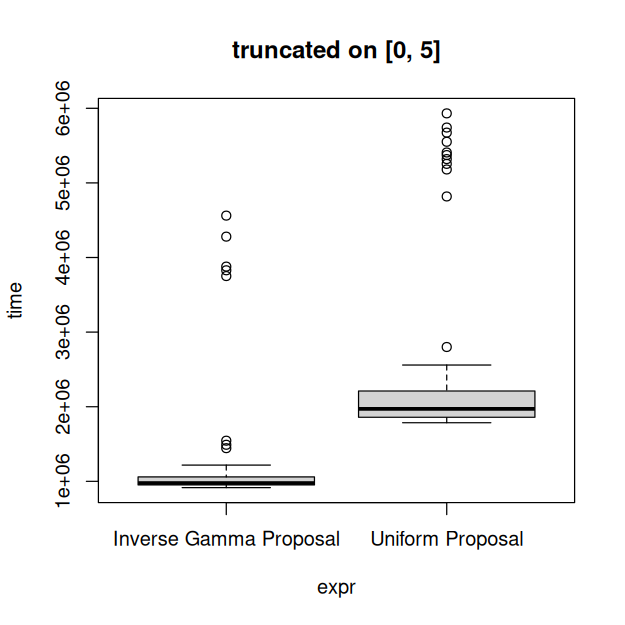
\includegraphics[width=0.48\columnwidth, height=0.3\columnwidth, keepaspectratio]{imgs/b_eq_5.png}%
    \hspace{0.01\columnwidth}%
    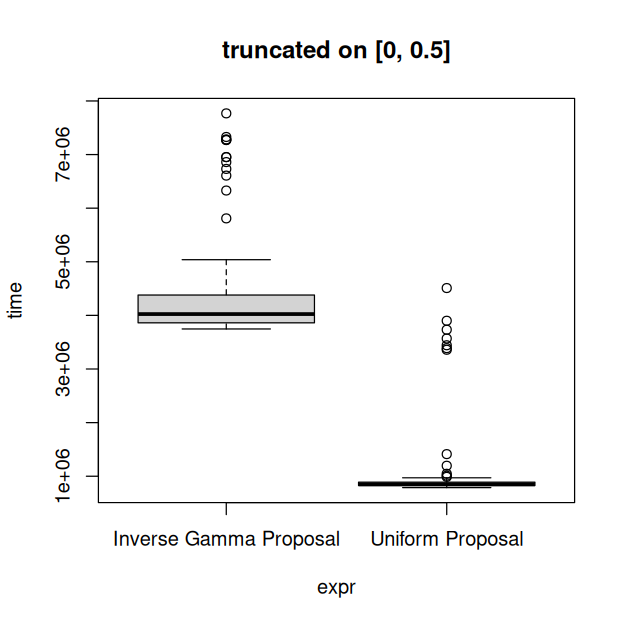
\includegraphics[width=0.48\columnwidth, height=0.3\columnwidth, keepaspectratio]{imgs/b_eq_05.png}
    \label{fig:performance}
\end{figure}

\vspace{-0.6cm}

For number of samples \(n = 10^4\), we can see that when \(b = 5\) (left), the inverse-gamma proposal sampler performs better than the uniform proposal sampler, using shorter time to generate samples and the generation time variance is also smaller. When \(b = 0.5\) (right), the uniform proposal sampler performs better, with both shorter time and smaller variance in time. This is explained by the optimal bounding constant \(M\) we calculated in Section 1.
% \[ M = \begin{cases}
%         \frac{1}{F_{\alpha, \beta}(b) - F_{\alpha, \beta}(0)} & \text{for inverse-gamma proposal} \\[0.5em]
%         \begin{cases}
%             \frac{b}{F_{\alpha, \beta}(b) - F_{\alpha, \beta}(0)} \times \frac{\beta^{\alpha}}{\Gamma(\alpha)} b^{-\alpha-1} \exp \left(-\frac{\beta}{b}\right), & b \leq \frac{\beta}{\alpha + 1} \\[1em]
%             \frac{b}{F_{\alpha, \beta}(b) - F_{\alpha, \beta}(0)} \times \frac{\beta^{\alpha}}{\Gamma(\alpha)} \left(\frac{\beta}{\alpha + 1}\right)^{-\alpha-1} \exp \left(-\frac{\alpha + 1}{1}\right), & b > \frac{\beta}{\alpha + 1}
%         \end{cases} & \text{for uniform proposal}
%     \end{cases} \]

\begin{lstlisting}
> (pinvgamma(5,3,2) - pinvgamma(0,3,2))^(-1)
[1] 1.00799 ## inverse-gamma proposal b = 5
> const <- 5/(pinvgamma(5,3,2) - pinvgamma(0,3,2)) * 2^3/gamma(3)
> const * (2/(3+1))^(-3-1) * exp(-3-1)
[1] 5.907832 ## uniform proposal b = 5

> (pinvgamma(0.5,3,2) - pinvgamma(0,3,2))^(-1)
[1] 4.199858 ## inverse-gamma proposal b = 0.5
> const <- 0.5/(pinvgamma(0.5,3,2) - pinvgamma(0,3,2)) * 2^3/gamma(3)
> const * 0.5^(-3-1) * exp(-2/0.5)
[1] 2.461538 ## uniform proposal b = 0.5
\end{lstlisting}
A smaller \(M\) leads to a higher acceptance rate in the rejection sampling, thus less time is needed to generate the required number of samples. Our calculations results is thus consistent with the observed performance of the two samplers in the experiments.